\documentclass[10pt, a4paper]{beamer}
\usepackage{graphicx}
\usetheme{Berlin}
\usecolortheme{seagull}
\begin{document}
	\setbeamertemplate{seagull left}{}
	\title{Progress Presentation-I}
	\subtitle{e-Yantra Summer Intership-2016 \\ Tiva based Daughter Board For Firebird V}
	\author{Ayush Gaurav \\Nagesh K \\ Mentors:\\ Piyush Manavar \\Saurav Shandilya \\}
	\institute{IIT Bombay}
	\date{\today}
	%\addtobeamertemplate{sidebar left}{}{\includegraphics[scale = 0.3]{logowithtext.png}}
	\frame{\titlepage}

\setbeamertemplate{sidebar left}[seagull theme]
\section{Overview of Project}
\begin{frame}{Overview of Project}
	\begin{itemize}
		\item Project Name: Tiva based Daughter Board For Firebird V.
		\item Objective: To design and develop a daughter board for firebird V with the following criterion:
			\begin{enumerate}
				\item Tiva Based Platform.
				\item On board Programing facility.
				\item Direct compatibility to Firebird.
			\end{enumerate}
		\item Deliverables:
		\begin{enumerate}
			\item Final schematic.\begin{itemize}
				\item Launchpad based daughter board 
				\item TM4C123GH6PM based daughter board
			\end{itemize}
			\item Working daughter board.
			\item Working codes for I/O, PWM, position encoders, lcd, wired and wireless communication, ADC.
		\end{enumerate}
	\end{itemize}
\end{frame}

\section{Overview of Task}
\begin{frame}{Overview of Task}
	\begin{tabular}{|c|c|c|}
		\hline
		 & & \\
		Task & Deadline & Status\\
		 & & \\
		\hline
		 & & \\
			 {Understaing daughter board.}& &\\
			{List the pins of daughter board.} & 3 days & Completed\\
			{Familiarize with Tiva C series Launchpad.} & &\\
			 & & \\
			\hline
			 & & \\
			Finalize the platform to design & 3 days & Completed\\
			 & & \\
			\hline
			 & & \\
			 Design the schematic. & 2 days & Completed \\
			 Check compatibality with Firebird. & & \\ 
			  & & \\
			\hline			
	\end{tabular}
\end{frame}

\section{Overview of Task}
\begin{frame}{Overview of Task}
\begin{tabular}{|c|c|c|}
	\hline
	& & \\
	Task & Deadline & Status\\
	& & \\
	\hline
	& & \\
	Discuss and add the necessary features & 3 days  & completed  \\ to achieve maximum functionality. & &  \\ 
	 & & \\
	\hline
	 & & \\
	Finalize the schematic. & 1 day & completed \\
	 & & \\
	\hline			
\end{tabular}
\end{frame}

\section{Task Accomplised}
\begin{frame}{Task Accomplised}
	\begin{itemize}
		\item Familiarization with Tiva Launchpad. Interfaced the following:
			\begin{itemize}
				\item GPIO
				\item Timers and its interrupts.
				\item External interrupts.
				\item Pulse Width Modulation.
				\item UART and its interrupts.
				\item Wired and wireless 
				\item Analog to digital converter.
				\item LCD.
			\end{itemize}
		\item Studied the circuits to run the micro-controller. 
		\item Analyzing the pins of firebird.
		\item Assigning the pins of uC.
		\item designing the schematics.
	\end{itemize}
\end{frame}
\section{Pin Assignment}
	\begin{frame}{Pin Assignment of uC based board}
		{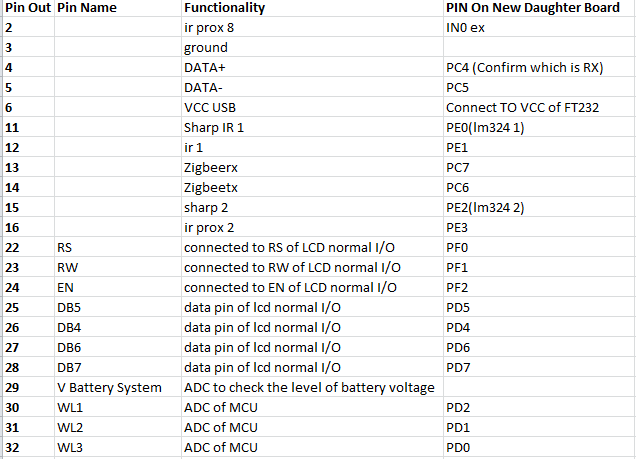
\includegraphics[width=10cm]{1.PNG}}
	\end{frame}
\section{Pin Assignment}
\begin{frame}{Pin Assignment of uC based board}
{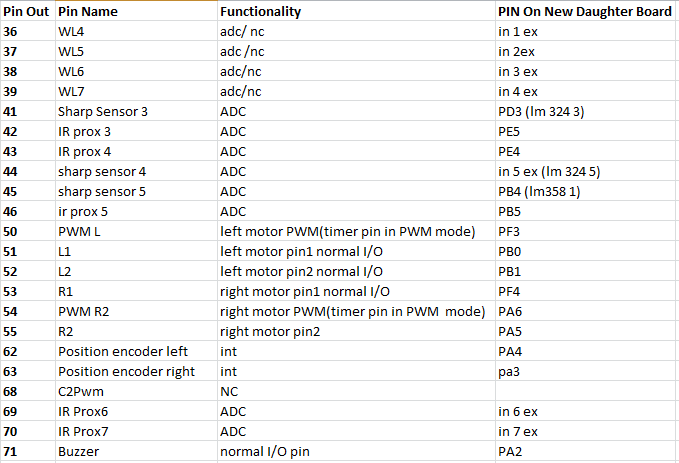
\includegraphics[width=10cm]{2.PNG}}
\end{frame}
\section{Pin Assignment}
\begin{frame}{Pin Assignment of launchpad based board}
{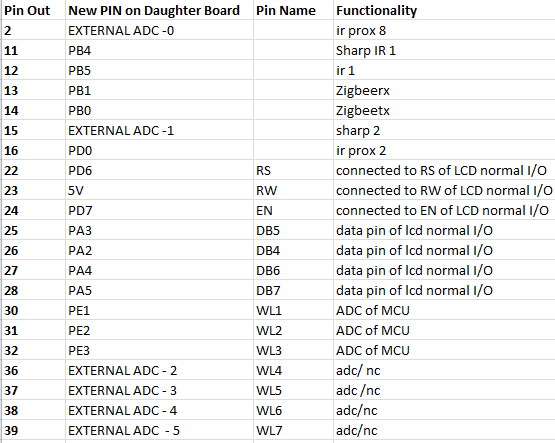
\includegraphics[width=10cm]{3.PNG}}
\end{frame}
\section{Pin Assignment}
\begin{frame}{Pin Assignment of launchpad based board}
{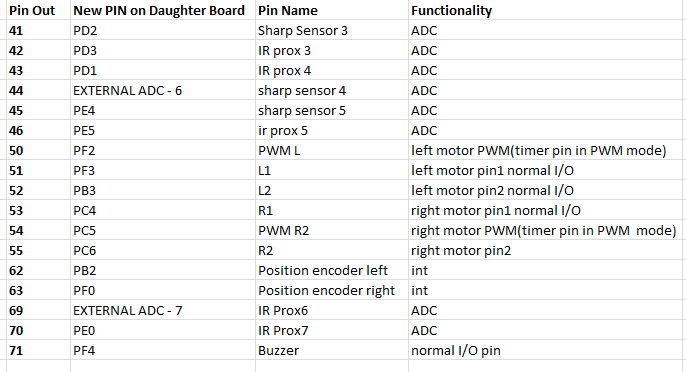
\includegraphics[width=10cm]{4.PNG}}
\end{frame}
\section{Schematic}
\begin{frame}{Schematic of uC based board}
{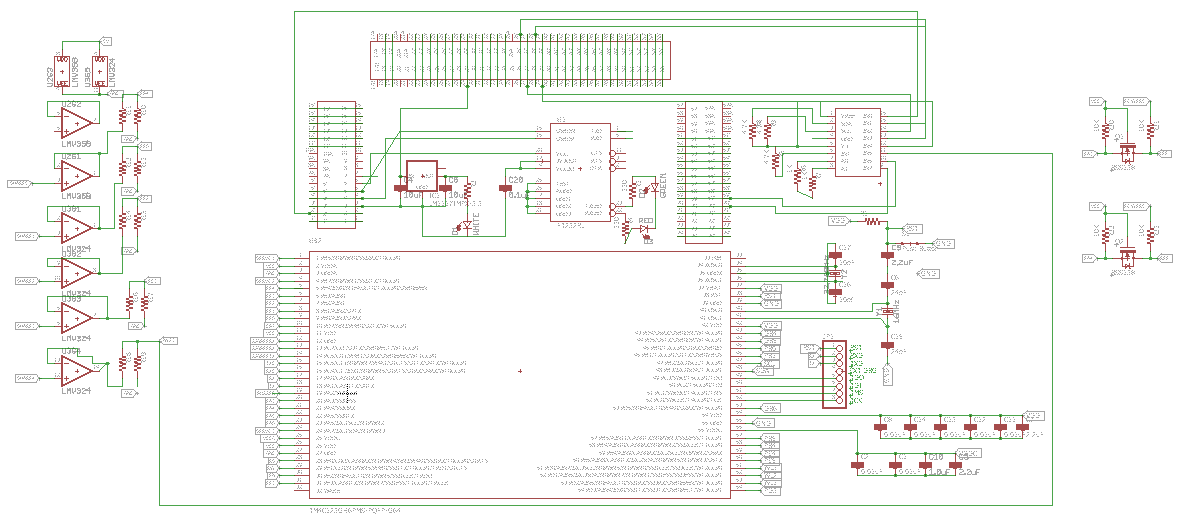
\includegraphics[width=12cm]{5.PNG}}
\end{frame}

\section{Schematic}
\begin{frame}{Schematic of launchpad based board}
{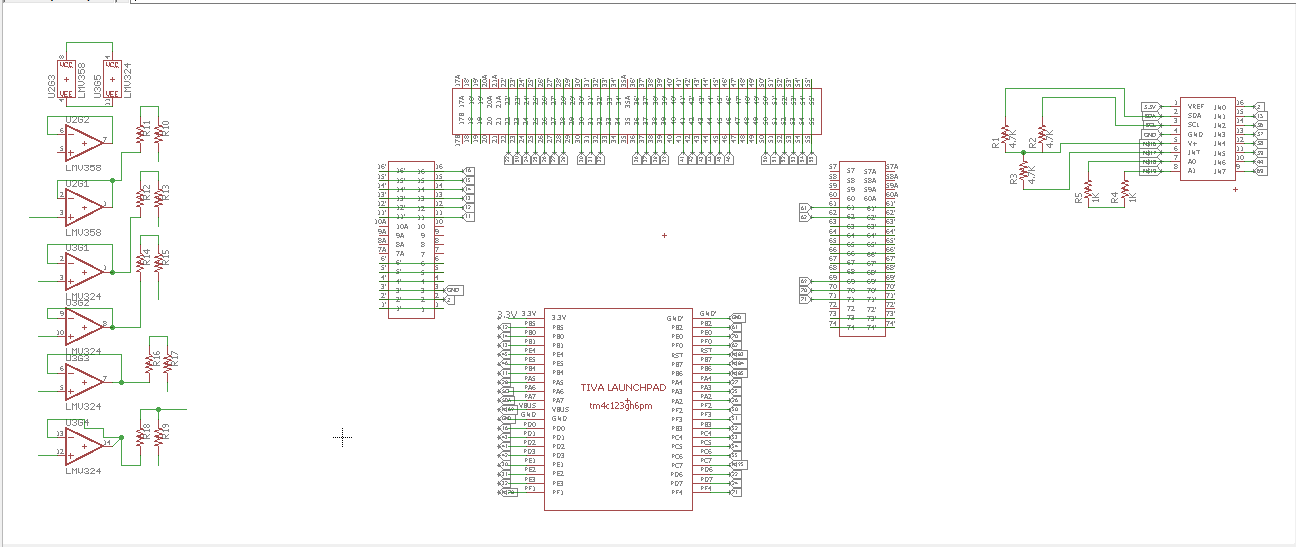
\includegraphics[width=12cm]{6.PNG}}
\end{frame}

\section{Layout}
\begin{frame}{Layout of launchpad based board}
{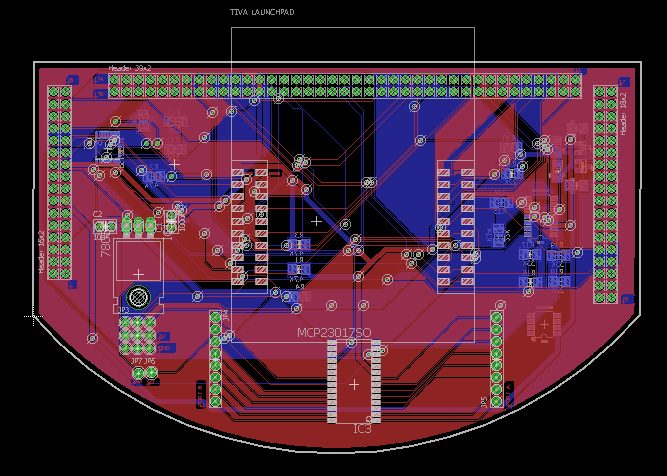
\includegraphics[width=10cm]{8.PNG}}
\end{frame}
\section{Layout}
\begin{frame}{Layout of uC based board}
{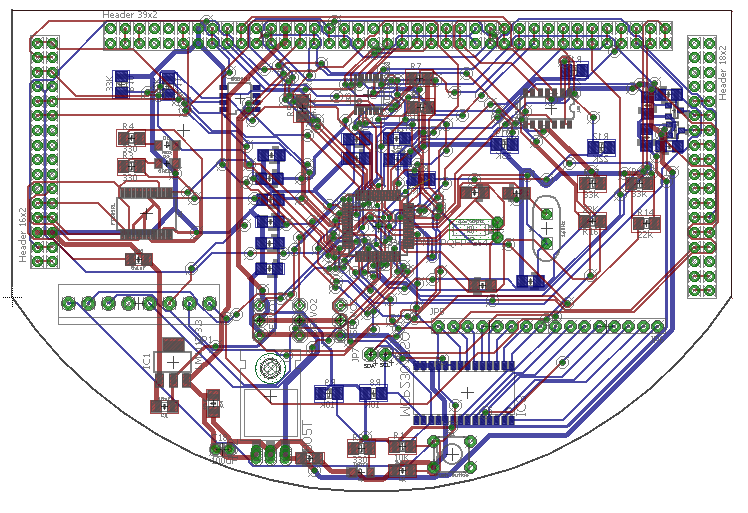
\includegraphics[width=10cm]{7.PNG}}
\end{frame}

\section{Challenges Faced}
\begin{frame}{Challenges Faced}
	\begin{itemize}
		\item Voltage incompatibility.
		\item Pin availability.
		\item number of sensors on firebird
		\item Nonavailability of firmware to program the board.
		\item Interfacing 5V compatible sensors with 3.3V compatible uC.
		\item Separate power supply for servo motors.
	\end{itemize}
\end{frame}

\section{Future Plans}
\begin{frame}{Future Plans}
	\begin{itemize}
		\item Working Daughter board in next 2 weeks.
		\item All the  working codes.
		\item Proper hardware manual by the end of the internship period.   
	\end{itemize}
\end{frame}


\section{Thank You}
\begin{frame}{Thank You}
	\centering THANK YOU !!!
\end{frame}
\end{document}
